\chapter{Результаты экспериментов}
\section{Оценка линейного искажающего оператора}
\begin{figure}[h!]
	\centering
	\begin{subfigure}[b]{0.475\textwidth}
		\centering
		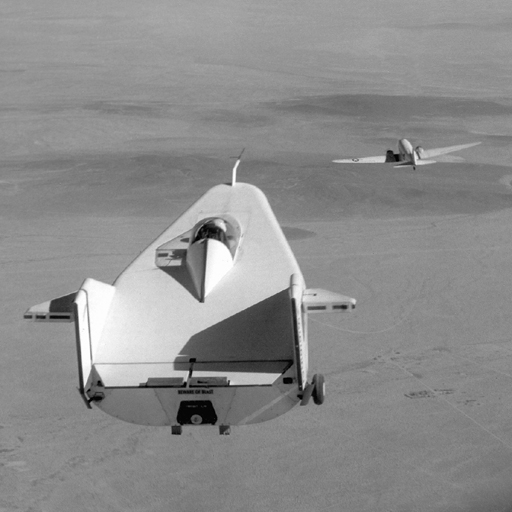
\includegraphics[width=\linewidth]{../liftingbody}
		\caption{исходное изображение}
		\label{fig:liftingbody}
	\end{subfigure}
	\hfill
	\begin{subfigure}[b]{0.475\textwidth}
		\centering
		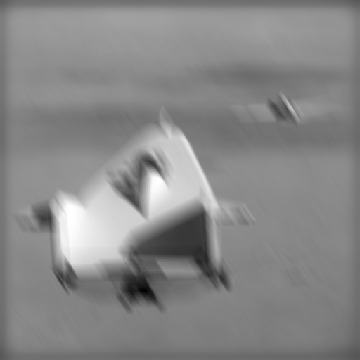
\includegraphics[width=\linewidth]{linear-lifting-blurred}
		\caption{Смазанное изображение. [16.67; 24.94]}
		\label{fig:liftingBlurred}
	\end{subfigure}
\vskip\baselineskip
	\begin{subfigure}[b]{0.475\textwidth}
	\centering
	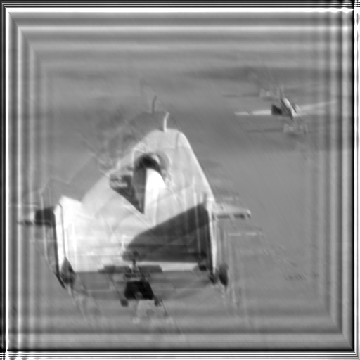
\includegraphics[width=\linewidth]{linear-restored-initial-approx}
	\caption{Первое приближение(по кепстру) [17; 25], PSNR=27.26дБ}
	\label{fig:liftingbodyInitial}
	\end{subfigure}
	\hfill
	\begin{subfigure}[b]{0.475\textwidth}
		\centering
		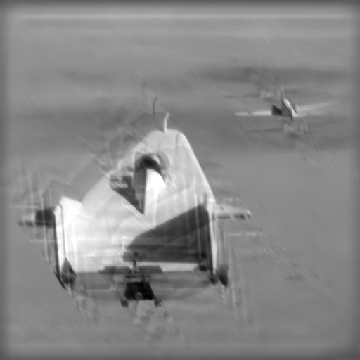
\includegraphics[width=\linewidth]{linear-restored-final}
		\caption{уточнённая оценка. [17.0006 25.0022], PSNR=27.26дБ}
		\label{fig:liftingFinal}
	\end{subfigure}
	\caption{Восстановление изображения подвергнутого линейному смазу}
	\label{fig:linear}
\end{figure}
Рассмотрим смаз длины 30, под углом $56.25^\circ$. Как видим оценка на основе кепстра сразу дала удовлетворительный результат, при этом дальнейшая попытка улучшения качества восстановления результат практически не изменила.

\section{Оценка криволинейного искажающего оператора}
\subsection{Искусственные искажения}
Пусть искажение представлено криволинейным смазом~\ref{fig:oneDimIterPsfTrue}:
\begin{figure}[h!]
	\begin{subfigure}[t]{0.45\textwidth}
		\centering
		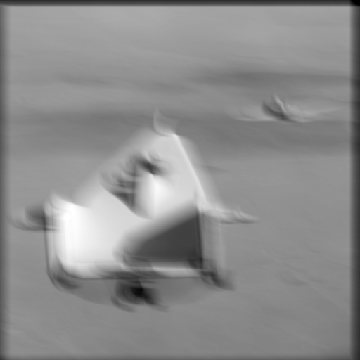
\includegraphics[width=\linewidth]{one-dim-iterated-blurred-data}
		\caption{смазанное изображение}
		\label{fig:oneDimIterBlurred}
	\end{subfigure}
	\hfill
	\begin{subfigure}[t]{0.45\textwidth}
		\centering
		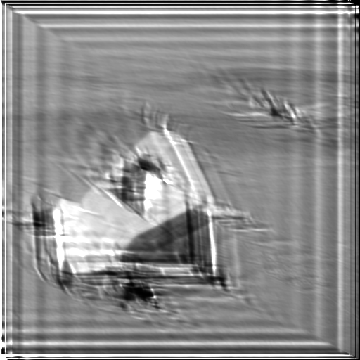
\includegraphics[width=\linewidth]{one-dim-iterated-restored-initial-approx}
		\caption{первое приближение: (0;0) (16;9) (32;18), PSNR=19.76дБ}
		\label{fig:oneDimIterInitial}
	\end{subfigure}

	\begin{subfigure}[t]{0.45\textwidth}
		\centering
		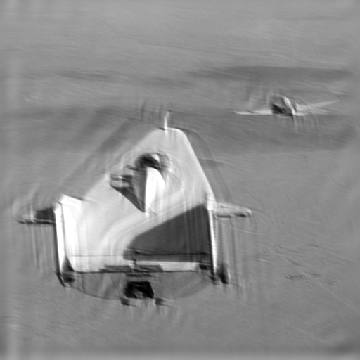
\includegraphics[width=\linewidth]{one-dim-iterated-restored-second-approx}
		\caption{первое приближение: (0;0) (7;25) (32;18), PSNR=26.44дБ}
		\label{fig:oneDimIterSecond}
	\end{subfigure}
	\hfill
	\begin{subfigure}[t]{0.45\textwidth}
		\centering
		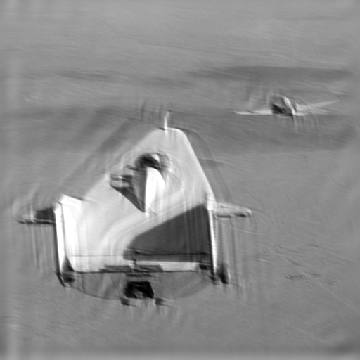
\includegraphics[width=\linewidth]{one-dim-iterated-restored-second-approx}
		\caption{первое приближение: (0;0) (7;25) (31.996;18.006), PSNR=27.29дБ}
		\label{fig:oneDimIterFinal}
	\end{subfigure}
	\caption{Восстановление изображения подвергнутого смазу оператором  оператором \ref{fig:oneDimIterPsfTrue}}
	\label{fig:oneDimIter}
\end{figure}
На рис.~\ref{fig:oneDimIter} показаны результаты деконволюции смазанного изображения с ИХ на различных этапах оценки. Как видим уже начальное приближение рис.~\ref{fig:oneDimIterInitial} повышает резкость. Набольший вклад в качество восстановления даёт второе приближение рис.~\ref{fig:oneDimIterSecond}. Последующее уточнение не сильно влияет на результат.

\begin{figure}[h!]
	\centering
	\begin{subfigure}[t]{0.475\textwidth}
		\centering
		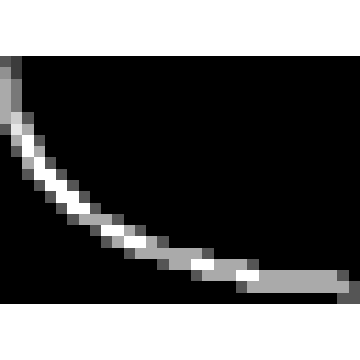
\includegraphics[width=\linewidth]{one-dim-iterated-curved-psf-real}
		\caption{криволинейная ИХ~--- кривая Безье: (0;0), (1; 18), (30, 20)}
		\label{fig:oneDimIterPsfTrue}
	\end{subfigure}
	\hfill
	\begin{subfigure}[t]{0.475\textwidth}
		\centering
		
\includegraphics[width=\linewidth]{one-dim-iterated-curved-psf-found}
		\caption{Оценка искажающего оператора: (0;0) (7;25) (31.996;18.006)}
		\label{fig:oneDimIterPsfFound}
	\end{subfigure}
	\caption{ИХ: действительная, и её оценка}
	\label{fig:oneDimIterPsf}
\end{figure}
Заметим, что оценка(рис.~\ref{fig:oneDimIterPsfFound}) искажающего оператора достаточно точно воспроизводит использованную для искажения ИХ(рис.~\ref{fig:oneDimIterPsfTrue}).

\subsection{Искажения <<от руки>>}

Смоделируем искажающий оператор, нарисовав кривую в графическом редакторе <<от руки>> рис.~\ref{fig:drawnPsf3}:
\begin{comment}
\begin{figure}[h!]
	\centering
	\begin{subfigure}[t]{0.475\textwidth}
		\centering
		
\includegraphics[width=\linewidth]{../input/drawn-psf}
		\caption{ИХ $h_1$}
		\label{fig:drawnPsf1}
	\end{subfigure}
	\hfill
	\begin{subfigure}[t]{0.475\textwidth}
		\centering
		
\includegraphics[width=\linewidth]{../input/drawn-psf2}
		\caption{ИХ $h_2$}
		\label{fig:drawnPsf2}
	\end{subfigure}

	\begin{subfigure}[t]{0.475\textwidth}
		\centering
		
\includegraphics[width=\linewidth]{../input/drawn-psf3}
		\caption{ИХ $h_3$}
		\label{fig:drawnPsf3}
	\end{subfigure}
	\hfill
	\begin{subfigure}[t]{0.475\textwidth}
		\centering
		
\includegraphics[width=\linewidth]{../input/drawn-psf4}
		\caption{ИХ $h_4$}
		\label{fig:drawnPsf4}
	\end{subfigure}
	\caption{Импульсные характеристики}
	\label{fig:drawnPsf}
\end{figure}
\end{comment}
\begin{figure}[h]
	\centering
	
\includegraphics[width=0.3\linewidth]{../input/drawn-psf3}
	\caption{ИХ $h$}
	\label{fig:drawnPsf3}
\end{figure}
Затем попробуем восстановить искажённые такими операторами изображения.

\begin{figure}[h!]
	\centering
	\begin{subfigure}[t]{0.475\textwidth}
		\centering
		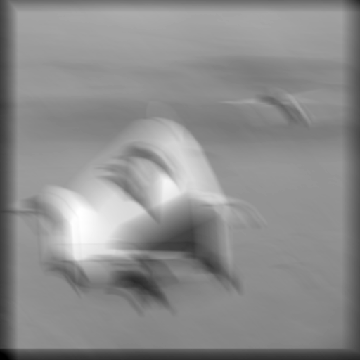
\includegraphics[width=\linewidth]{one-dim-drawn-lifting-blurred}
		\caption{смазанное изображение}
		\label{fig:oneDimDrawnLiftingBlurred}
	\end{subfigure}
	\hfill
	\begin{subfigure}[t]{0.475\textwidth}
		\centering
		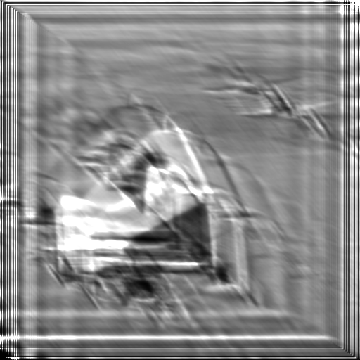
\includegraphics[width=\linewidth]{one-dim-drawn-restored-initial-approx}
		\caption{восстановленное, первое приближение (0;0) (26;17) (52;34), PSNR=19.18дБ}
		\label{fig:oneDimDrawnLiftingInitial}
	\end{subfigure}


	\begin{subfigure}[t]{0.475\textwidth}
		\centering
		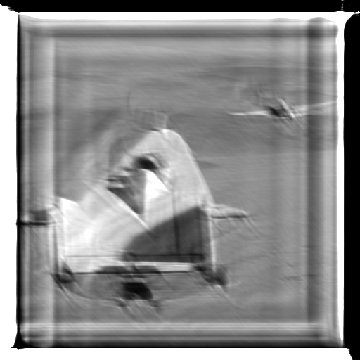
\includegraphics[width=\linewidth]{one-dim-drawn-restored-second-approx}
		\caption{второе приближение (0;0), (40.66;-5.41), (52;34), PSNR=22.25дБ}
		\label{fig:oneDimDrawnLiftingSecond}
	\end{subfigure}
	\hfill
	\begin{subfigure}[t]{0.475\textwidth}
		\centering
		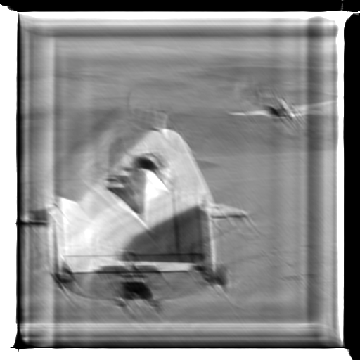
\includegraphics[width=\linewidth]{one-dim-drawn-restored-final}
		\caption{уточнение градиентным спуском (0,0), (40.65;-5.43), (52, 34), PSNR=22.37}
		\label{fig:oneDimDrawnLiftingFinal}
	\end{subfigure}
	\caption{Восстановление изображения искажённого оператором \ref{fig:drawnPsf3}}
	\label{fig:oneDimDrawnLifting}
\end{figure}
На рисунке \ref{fig:oneDimDrawnLifting} изображён процесс восстановления изображения, искажённого нарисованным <<от руки>> оператором. Как и в предыдущем случае наибольший вклад в качество восстановленного изображения внесли первое и второе приближение оценки параметров оператора.

\begin{figure}[h!]
	\centering
	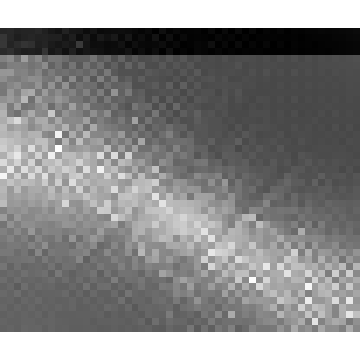
\includegraphics[width=0.4\linewidth]{one-dim-drawn-lifting-cost-function-grid}
	\caption{Значения целевой функции в зависимости от координат второй точки}
	\label{fig:drawnCostFunction}
\end{figure}
На рисунке~\ref{fig:drawnCostFunction} показано представление целевой функции в зависимости от координат второй точки$B_1$ кривой Безье. Как видим в данном случае так же большое количество локальных минимумов(тёмных пикселей окружённых светлыми).

\begin{figure}[h!]
	\centering
	\begin{subfigure}[t]{0.475\textwidth}
		\centering
		
\includegraphics[width=0.3\linewidth]{../input/drawn-psf3}
		\caption{ИХ $h$}
		\label{fig:drawnPsf3Orig}
	\end{subfigure}
	\begin{subfigure}[t]{0.15\textwidth}
		\centering
		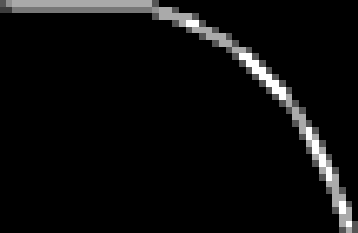
\includegraphics[width=\linewidth]{one-dim-drawn-lifting-psf-found}
		\caption{оценка $\hat{h}$}
		\label{fig:drawnPsf3Estimation}
		
	\end{subfigure}
	\caption{Искажающий оператор и его оценка кривой Безье}
	\label{fig:drawnPsf3Est}
\end{figure}
Полученная оценка(рис.~\ref{fig:drawnPsf3Estimation}) искажающего оператора(рис.~\ref{fig:drawnPsf3Orig}) полученная из смазанного изображения хорошо описывает искажение и позовляет получить достаточно чётко восстановленное изображение.
\begin{comment}

\begin{figure}[h!]
	\centering
	\begin{subfigure}[t]{0.475\textwidth}
		\centering
		\includegraphics[width=\linewidth]{***}
		\caption{***}
		\label{fig:***}
	\end{subfigure}
	\hfill
	\begin{subfigure}[t]{0.475\textwidth}
		\centering
		\includegraphics[width=\linewidth]{***}
		\caption{***}
		\label{fig:***}
	\end{subfigure}
	\caption{***}
	\label{fig:***}
\end{figure}

\end{comment}

\section{Выводы}
Все эксперименты и предложенные методы были реализованы в среде jupyter-notebook с ядром python3.6. По результатам экспериментов были сделаны следующие выводы
\begin{enumerate}
	\item Метод Люси-Ричардсона позволяет получить более качественный результат по сравнению с другими методами;
	\item разработан метод оценки криволинейного искажающего оператора;
	\item применение кепстрального представления позовляет определить параметры не только прямолинейного искажающего оператора, но и первое приближение для криволинейного оператора;
	\item для повышения точности оценки параметров искажения следует использовать минимизацию функции ошибки, которая является <<плохой>> для градиентных методов, но поддаётся минимизации, с учётом модели искажения.
	\item результат работы первого и второго приближения даёт приемлемый результат, тогда как попытки градиентными методами минимизации целевой функции на результат большого влияния не оказывают. Таким образом исключив последний этап можно значительно ускорить работу алгоритма с небольшими потерями в точности восстановления;
\end{enumerate}